\clearpage
\newpage
\begin{figure}[H]
 \begin{algorithm}[H]
 	\SetAlgorithmName{Generative Process}
 	\DontPrintSemicolon
 	\SetAlgoNoLine
 	\KwIn{$N,n,R,\{\lambda_t\}_{t\in\Tc},\Tc= 
 		\{\tau_0,\ldots\tau_T\}$ }
 	\KwOut{Time-series pool-seq data for $R$ replicates of a single locus 
 		$\{\bfc\}_R$ and $\{\bfd\}_R$.}
 	\For{$r\leftarrow 1$ \KwTo $R$}
 	{
 		\For{$t\leftarrow \tau_0$ \KwTo $\tau_T$}
 		{
 			$2N\nu_t \sim \text{Binomial}({2N},{\nu_{t-1}})$\;
 			\If{$t\in \Tc$ }
 			{
 				$d^{(r)}_{t} \sim \poiss(\lambda_{\tau_i})$ \;
 				$2ny_t \sim \text{Binomial}({2n},{\nu_{t}})$\;  
 				$c^{(r)}_{t} \sim \text{Binomial}(d^{(r)}_{t},{y_{t}})$\; 
 			}
 		}
 	}
 	\caption{The Generative Process for Neutral Wright-Fisher 
 	Time-series Pool-seq Data.} 
 \end{algorithm}
 \caption{{\bf The Generative Process for Neutral Wright-Fisher 
 		Time-series Pool-seq Data.}}
  	\label{proc:arya}
\end{figure}	
\begin{figure}[H]
	\centering
	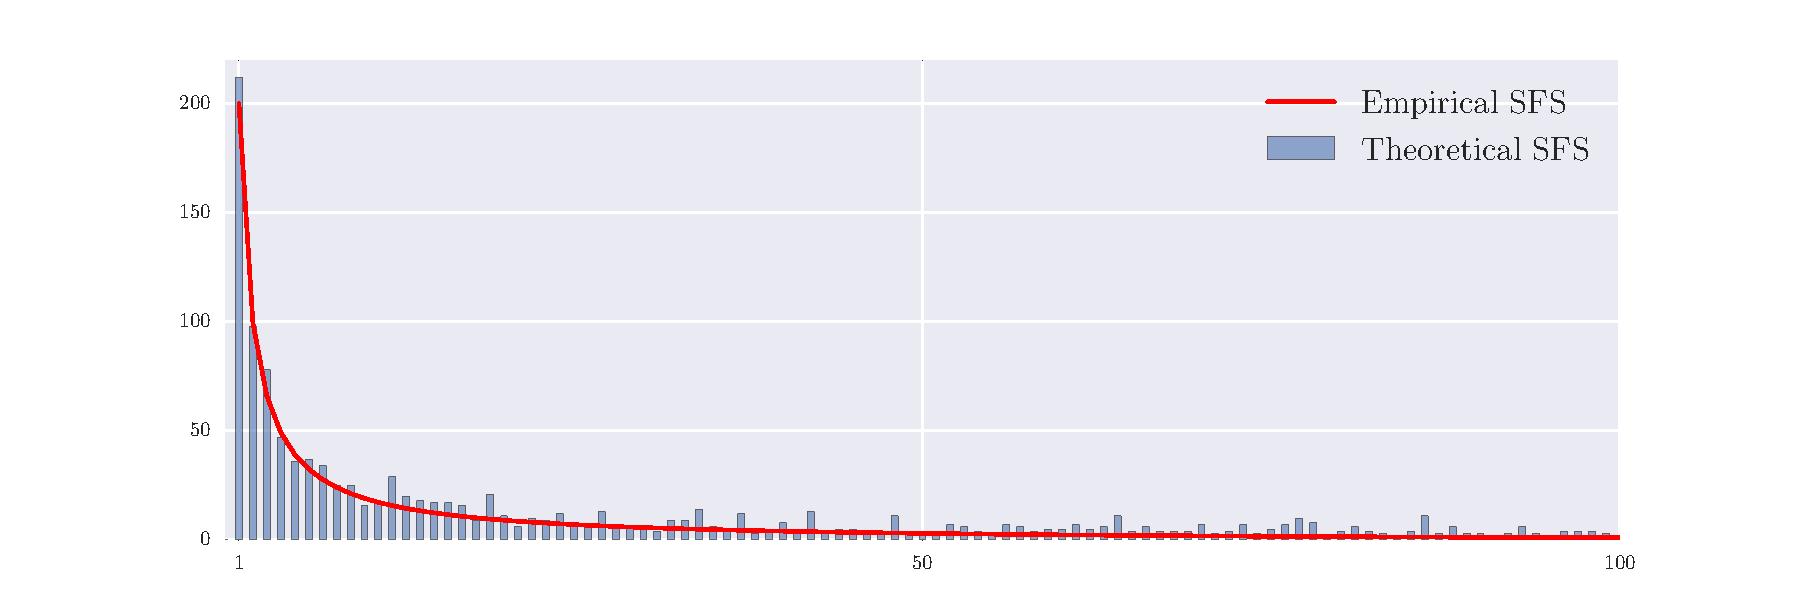
\includegraphics[trim=.01in 0.1in .01in 
	0.1in,clip,width=\textwidth]{sfs.pdf}
	\caption{{\bf Site Frequency Spectrum.}\\ Theoretical and
          Empirical SFS in a 50Kbp region for a neutral population of 200
          individuals when $N_e=10^6$ and $\mu=10^{-9}$. The $x$-axis 
          corresponds to site frequency, and
          the $y$-axis to the number of variants with a specific
          frequency. 
          In a neural population, majority of the variations stand in low 
          frequency.} \label{fig:sfs}
\end{figure}

\ignore{
\begin{figure}[H]
	\centering
	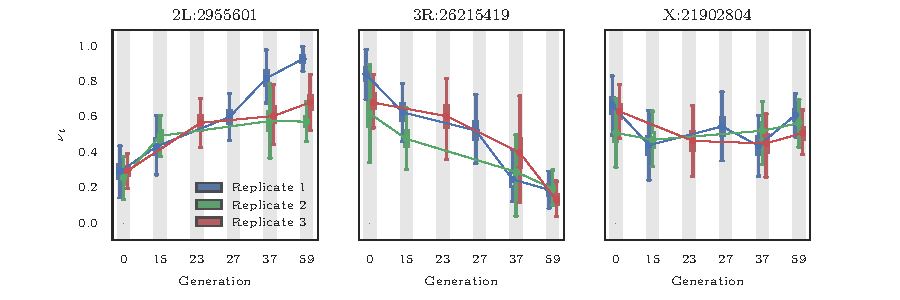
\includegraphics[width=\textwidth]{trajectoryReal.pdf}
	\caption{{\bf Trajectory of pool-sequenced variants.}\\
		Trajectory of three different variants that are increasing
		in frequency over time. Note that for read count data, the
		true allele frequency is not known. Here we draw the
		posterior distribution of the allele frequency at each time
		point using box plot. The median of each distribution is
		denoted by dots. The variance of each box is seen to be
		inversely related to the depth of the measurement. For instance, 
		generation 59 is sequenced with higher coverage than generation 37. 
		As a result, variance of observations in generation 59 is 
		considerably 
		smaller.}
	\label{fig:trajectoryReal}
\end{figure}
\begin{figure}[H]
	\centering
	\includegraphics[trim=.0in 0 .0in 0, 
	clip,width=0.5\textwidth]{{statePosterior}.pdf}
	\caption{{\bf Posterior distribution of allele frequency.}\\
		Distribution of hidden allele frequency for different values
		of depth $d=\{5,50,500\}$. In all cases, the true frequency
		is $0.2$. The estimated frequency values are binomially distributed, 
		with different variances,
		around the true value in all cases with.}
	\label{fig:stateConditional}
\end{figure}}
\begin{figure}[H]
	\centering
	\begin{tabular}{c}
		\includegraphics[trim=.2in 0 .0in 0, 
		clip,width=0.8\textwidth]{{depthHetero}.pdf}
	\end{tabular}
	\caption{{\bf Coverage heterogeneity in time series data.}\\ Each panel
		shows the read depth for 3
		replicates of the \datadm\ data (see section~\ref{sec:dmel}). 
		Heterogeneity in depth of coverage is 
		seen
		between replicates, and also at different time points, in
		all 4 variants. None of these sites pass the the hard filtering with 
		minimum depth of 30. }
	\label{fig:depthHetero}
\end{figure}


\begin{figure}[H]
	\centering
	\includegraphics[width=0.6\textwidth]{{slikes}.pdf}
	\caption{{\bf Likelihoods of the parameter $s$.}\\ 
		Likelihood of the parameter $s$ in \dmel data for a variant with 
		$\hs=0.2$ (A) and $\hs=0$ (B). 
		}
	\label{fig:slikes}
\end{figure}


\begin{figure}[H]
	\centering
		\includegraphics[width=0.6\textwidth]{{bias.30}.pdf}
	\caption{{\bf Distribution of bias for 30$\times$ coverage.}\\ The
		distribution of bias ($s-\hat{s}$) in estimating selection
		coefficient over 1000 simulations using Gaussian Process (GP) and
		\comale\ ($H$) is shown for a range of choices for the selection
		coefficient $s$ and starting carrier frequency $\nu_0$, when
		coverage $\lambda=30$ (Panels A,B). GP and \comale\ have similar
		variance in estimates of $s$ for soft sweep, while \comale\ provides
		lower variance in hard sweep. Also see \ref{tab:biasdist}. Panels 
		C,D
		show the variance in the estimation of $h$.}
	\label{fig:bias30}
\end{figure}


\begin{figure}[H]
	\centering
	\includegraphics[width=0.6\textwidth]{{bias.300}.pdf}
	\caption{{\bf Distribution of bias for 300$\times$ coverage.}\\ The
		distribution of bias ($s-\hat{s}$) in estimating selection
		coefficient over 1000 simulations using Gaussian Process (GP) and
		\comale\ ($H$) is shown for a range of choices for the selection
		coefficient $s$ and starting carrier frequency $\nu_0$, when
		coverage $\lambda=\infty$ (Panels A,B). GP and \comale\ have similar
		variance in estimates of $s$ for soft sweep, while \comale\ provides
		lower variance in hard sweep. Also see \ref{tab:biasdist}. Panels 
		C,D
		show the variance in the estimation of $h$.
	}
	\label{fig:biasinf}
\end{figure}
\ignore{
\begin{figure}[H]
	\centering
	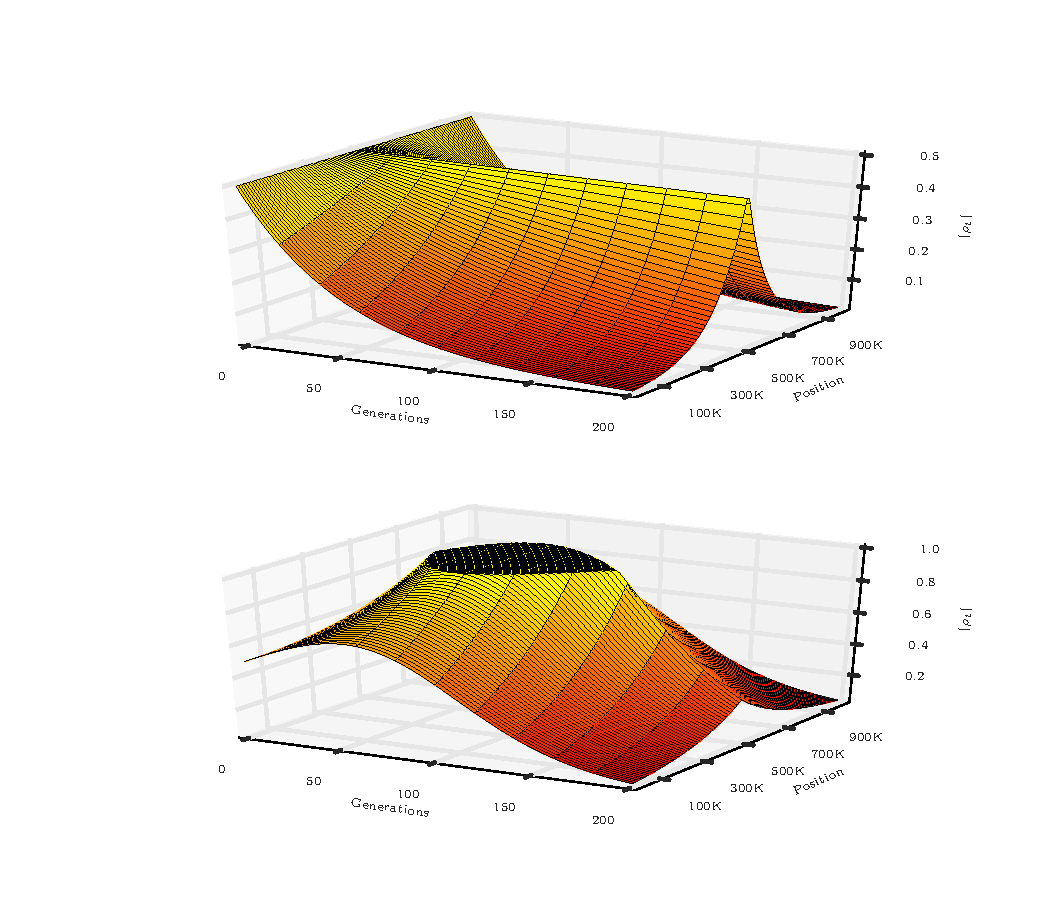
\includegraphics[width=\textwidth]{LDDecay3d}
	\caption{ {\bf Expected dynamic of LD under selection and neutral 
	evolution.}\\ Dynamic of LD ($\rho_t$) of a 1Mbp genome to the favored 
	allele 
	(at position 500K) is drawn as function of position and time for neutral 
	(top) and selection(bottom) regimes.
	For sake of illustration, we assumed that at generations 0, LD of all 
	variants with the favored allele is 0.5, initial frequency of the favored 
	allele is 0.1, recombination rate is $r=2\times10^{-8}$ (top). The 
	selection strength is 0 and 0.05 for neutral and selection regimes, 
	respectively. As expected LD decay exponentially  through space and time. 
	However, selection causes LD to increase then decrease.}	
		\label{fig:ld3d}
\end{figure}
}

\begin{figure}[H]
	\centering
		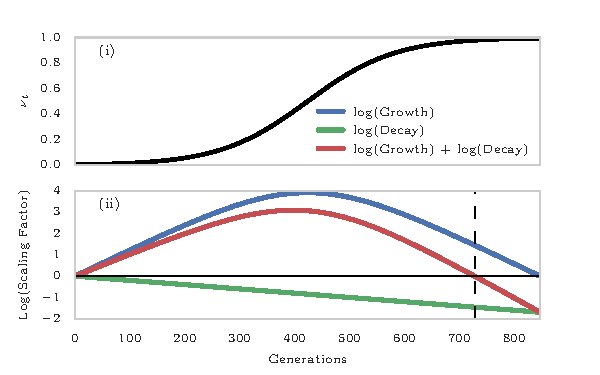
\includegraphics[width=0.8\textwidth]{decayFactors0}	
	\caption{{\bf Interaction between growth and decay factors of LD in 
	hard 
	sweep with	weak selection.}\\
		Expected dynamics of LD between favored allele and a variant 
		50Kbp 
		away, under weak selection ($s=0.025$) and hard 
		sweep 
		($\nu_0=0.005$). In addition to 
		recombination, initial frequency of the favored allele and selection 
		strength determine the dynamics of LD.
		The horizontal black line denotes the equilibrium between decay 
		and scaling factor.
		 The vertical dashed line represent the time in which decay and 
		 growth factors stay at equilibrium, after onset of selection.} 
		 \label{fig:ldf0}
\end{figure}

\begin{figure}[H]
	\centering
	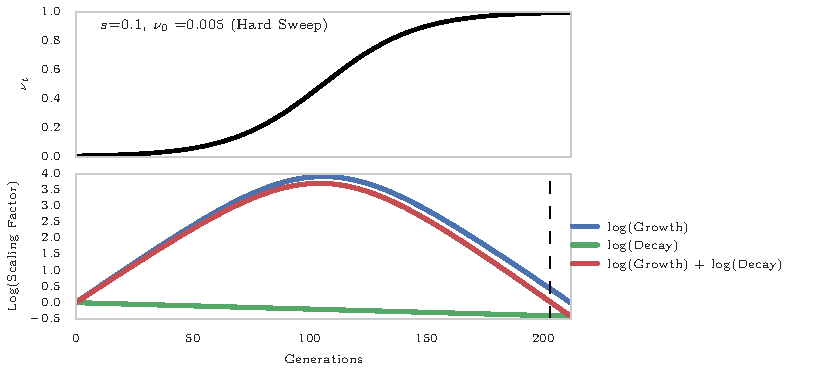
\includegraphics[width=0.8\textwidth]{decayFactors1}	
\caption{{\bf Interaction between growth and decay factors of LD in 
hard 
		sweep with	strong selection.}\\
	Expected dynamics of LD between favored allele and a variant 50Kbp 
	away, under strong selection ($s=0.1$) and hard sweep 
	($\nu_0=0.005$). In addition to 
	recombination, initial frequency of the favored allele and 
	selection 
	strength determine the dynamics of LD. The vertical dashed line 
	denotes 
	the time in which LD start to decrease. 		The horizontal 
	black line denotes the equilibrium between decay 
	and scaling factor.
	The vertical dashed line represent the time in which decay and 
	growth factors stay at equilibrium, after onset of selection.} 
	\label{fig:ldf1}
\end{figure}
\begin{figure}[H]
	\centering
	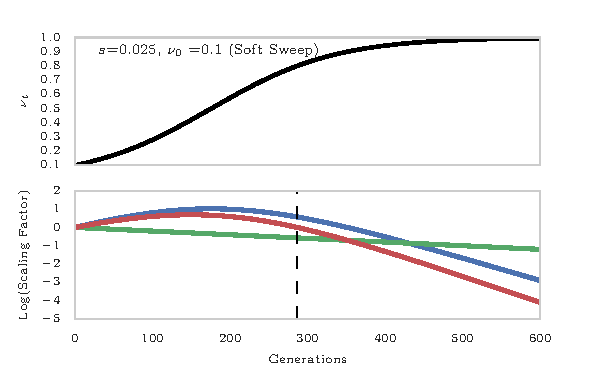
\includegraphics[width=0.8\textwidth]{decayFactors2}	
\caption{{\bf Interaction between growth and decay factors of LD in 
soft 
		sweep with	weak selection.}\\
	Expected dynamics of LD between favored allele and a variant 50Kbp 
	away, under weak selection ($s=0.025$) and soft sweep 
	($\nu_0=0.1$).  In addition to 
	recombination, initial frequency of the favored allele and 
	selection 
	strength determine the dynamics of LD. The vertical dashed line 
	denotes 
	the time in which LD start to decrease. 		The horizontal 
	black line denotes the equilibrium between decay 
	and scaling factor.
	The vertical dashed line represent the time in which decay and 
	growth factors stay at equilibrium, after onset of selection.} 
	\label{fig:ldf2}
\end{figure}
\begin{figure}[H]
	\centering
	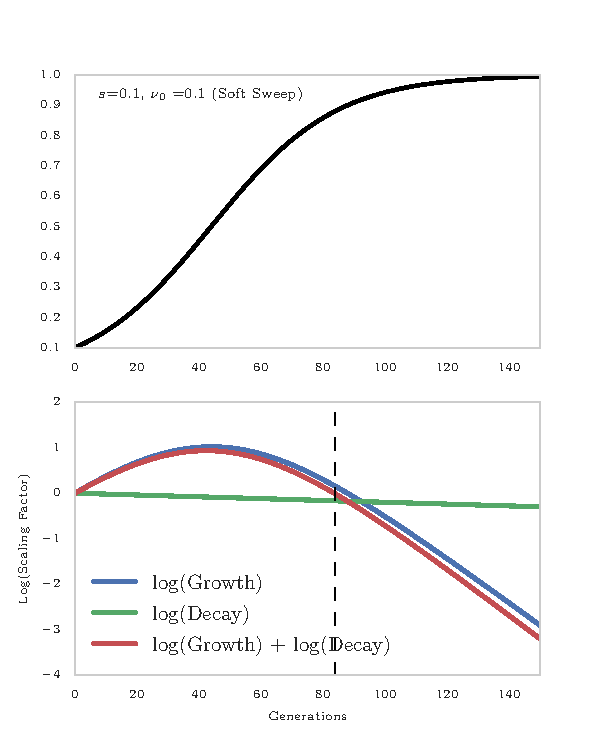
\includegraphics[width=0.8\textwidth]{decayFactors3}	
\caption{{\bf Interaction between growth and decay factors of LD in 
soft 
		sweep with	strong selection.}\\
	Expected dynamics of LD between favored allele and a variant 50Kbp 
	away, under strong selection ($s=0.1$) and soft sweep 
	($\nu_0=0.1$).  In addition to 
	recombination, initial frequency of the favored allele and 
	selection 
	strength determine the dynamics of LD. The vertical dashed line 
	denotes 
	the time in which LD start to decrease. 		The horizontal 
	black line denotes the equilibrium between decay 
	and scaling factor.
	The vertical dashed line represent the time in which decay and 
	growth factors stay at equilibrium, after onset of selection.} 
	\label{fig:ldf3}
\end{figure}


\begin{figure}[H]
	\centering
	\includegraphics[trim=.2in 0 .2in 0, 
	clip,width=\textwidth]{{rank30.0}.pdf}
	\caption{{\bf Ranking performance for 30$\times$ coverage.}\\
           Cumulative Distribution Function (CDF) of the distribution
           of the rank of the favored allele in 1000 simulations for
           \comale\ ($H$ score), Gaussian Process (GP), and Cochran 
           Mantel 
           Haenszel  
           (CMH), for different values of selection
           coefficient $s$ and initial carrier frequency.}
	\label{fig:rank300}
\end{figure}
\begin{figure}[H]
	\centering
	\includegraphics[trim=.2in 0 .2in 0, 
	clip,width=\textwidth]{{rank300.0}.pdf}
	\caption{{\bf Ranking performance for 300$\times$ coverage.}\\
           Cumulative Distribution Function (CDF) of the distribution
           of the rank of the favored allele in 1000 simulations for
           \comale\ ($H$ score), Gaussian Process (GP), and Cochran 
           Mantel 
           Haenszel  
           (CMH), for different values of selection
           coefficient $s$ and initial carrier frequency.}
	\label{fig:rankinf}
\end{figure}


\begin{figure}[H]
	\centering
	\includegraphics[width=0.7\textwidth]{{winSize}.pdf}
	\caption{{\bf Window size for $Ns$.}
Heuristic window size as function of $Ns$ for \dmel study with 
$\tau=59,N=250,r=2\times10^{-8}$.
	}
	\label{fig:winSize}
\end{figure}








\begin{figure}[H]
	\centering
	\includegraphics[trim=.0in 0in .2in 0in, 	
	clip,width=0.9\textwidth]{{null-alt-dmel}.pdf}
	\caption{{\bf Distribution of $p$-values.}
		Distribution of $p$-values of \comale\ in null simulations and 
		experimental data when $N=250$. Panel (A),(C) shows the effect of under 
		estimations ($\hN=100$) and over-estimation ($\hN=500$) of population 
		size in computing $p$-values, and panel (B) shows the distribution of 
		$p-$values when unbiased estimate is used to create simulations.
		.}
	\label{fig:null-alt}
\end{figure}


\begin{figure}[H]
	\centering
	\begin{tabular}{cc}
		(A)&(B)\\
		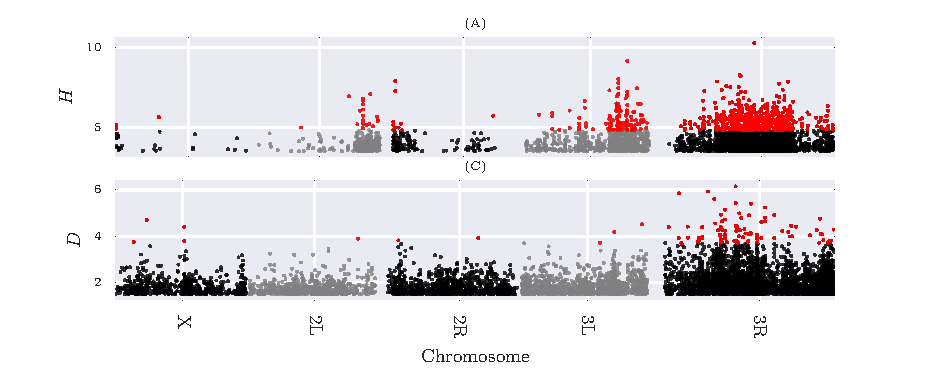
\includegraphics[trim=0.4in 0.in 0.6in 
		1.17in,clip,width=0.6\textwidth]{man-dmel-snp.pdf}&	
		\includegraphics[trim=0.1in 0.in 0in 
		1.5in,clip,width=0.35\textwidth]{{topVariants.dmel}.pdf}
	\end{tabular}
	\caption{{\bf Single locus analysis of the \datadm.}\\
	Manhattan plot of scan for
		testing dominant selection (A).  Significant variants
		with FDR $\le 0.01$ are denoted in red, and their
		trajectories are depicted in panel (B).}
	\label{fig:man-dmel-snp}
\end{figure}

\begin{figure}[H]
\begin{tabular}{cc}
	\includegraphics[width=0.5\textwidth]{{SFS.Y.G0}.pdf}&
	\includegraphics[width=0.5\textwidth]{{SFS.Y.G180}.pdf}\\
	\includegraphics[width=0.5\textwidth]{{SFS.Y.G360}.pdf}&
	\includegraphics[width=0.5\textwidth]{{SFS.Y.G540}.pdf}
\end{tabular}
\caption{{\bf Site frequency spectrum of the Yeast dataset.}
	Whole-genome site frequency spectrum of the Yeast dataset at generations 0 
	(A), 180 (B), 
	360 (C) and 540 (D). Some replicates, e.g. replicate 2, undergoing severe 
	demographic events.
	}
\label{fig:yeast-sfs}
\end{figure}

\begin{figure}[H]
	\centering
		\includegraphics[width=0.7\textwidth]{{PCA}.pdf}
	\caption{{\bf Population similarity.}
		Principle component analysis of the 12 replicates throughout the 
		experiment, showing that some populations exhibiting distinct frequency 
		spectra.
		}
	\label{fig:yeast-pca}
\end{figure}





